\documentclass[oneside]{report}
\usepackage{geometry}
\usepackage[english]{babel}
\usepackage[final]{graphicx}
\usepackage{amsmath}
\setlength{\parindent}{0pt}
\usepackage{float}
%\counterwithout{section}{chapter}
\usepackage{fullpage}
%\geometry{hmargin=20mm, vmargin=20mm}

\usepackage[backend=bibtex,
    natbib=true,
    style=numeric,
    sorting=none]{biblatex}
\addbibresource{lms464.bib} 

\begin{document}
\section*{Application Description}

Synaptic membranes are unique mammalian membranes \cite{Bozek2015}, composed of lipids that include a high fraction of omega-3 polyunsaturated fatty acids (PUFAs) and cholesterol \cite{Isolated1969,Breckenridge1973,Ingolfsson2017a}.  Pathologies that result in altered lipid composition of the neuronal membrane can have devastating effects, including Alzheimer's Disease, Parkinson's Disease, schizophrenia, and epilepsy \cite{MuralikrishnaAdibhatla}. As an example,  %people who suffered from Alzheimer's disease often have much lower levels of cholesterol in the membranes of their hippocampus than people without neurodegenerative disorders, and 
one of the most significant Alzheimer's disease risk factors is the $\epsilon$4 mutation in apolipoprotein E, which mediates cholesterol delivery to neurons.\cite{liu2013}\\

A major obstacle in understanding and treating all lipid-associated neurological disorders is that we do not understand how changing the lipid composition changes the behavior of neuronal membranes.  Molecular simulations are promising but have been limited in size and complexity.  The total synaptic apposition area is about 0.1-4$\mu$m$^{2}$\cite{yeow1991} with hundreds of lipids and proteins, while simulated membranes using coarse-grained models are about $10^{-4}\mu$m$^{2}$, and may contain a handful of lipids and one type of protein (Figure 1). \\

We are requesting an allocation for molecular simulations of neuronal cell membranes that are 100 times larger in area (Figure \ref{fig:Sci}B) and 10 times more complex than previous simulations conducted by any research group. These neuronal membranes will be 0.01 $\mu$m$^{2}$, with 30 species of lipid, 100 proteins, and 8 million particles. \\

\begin{figure}[h]
\begin{center}
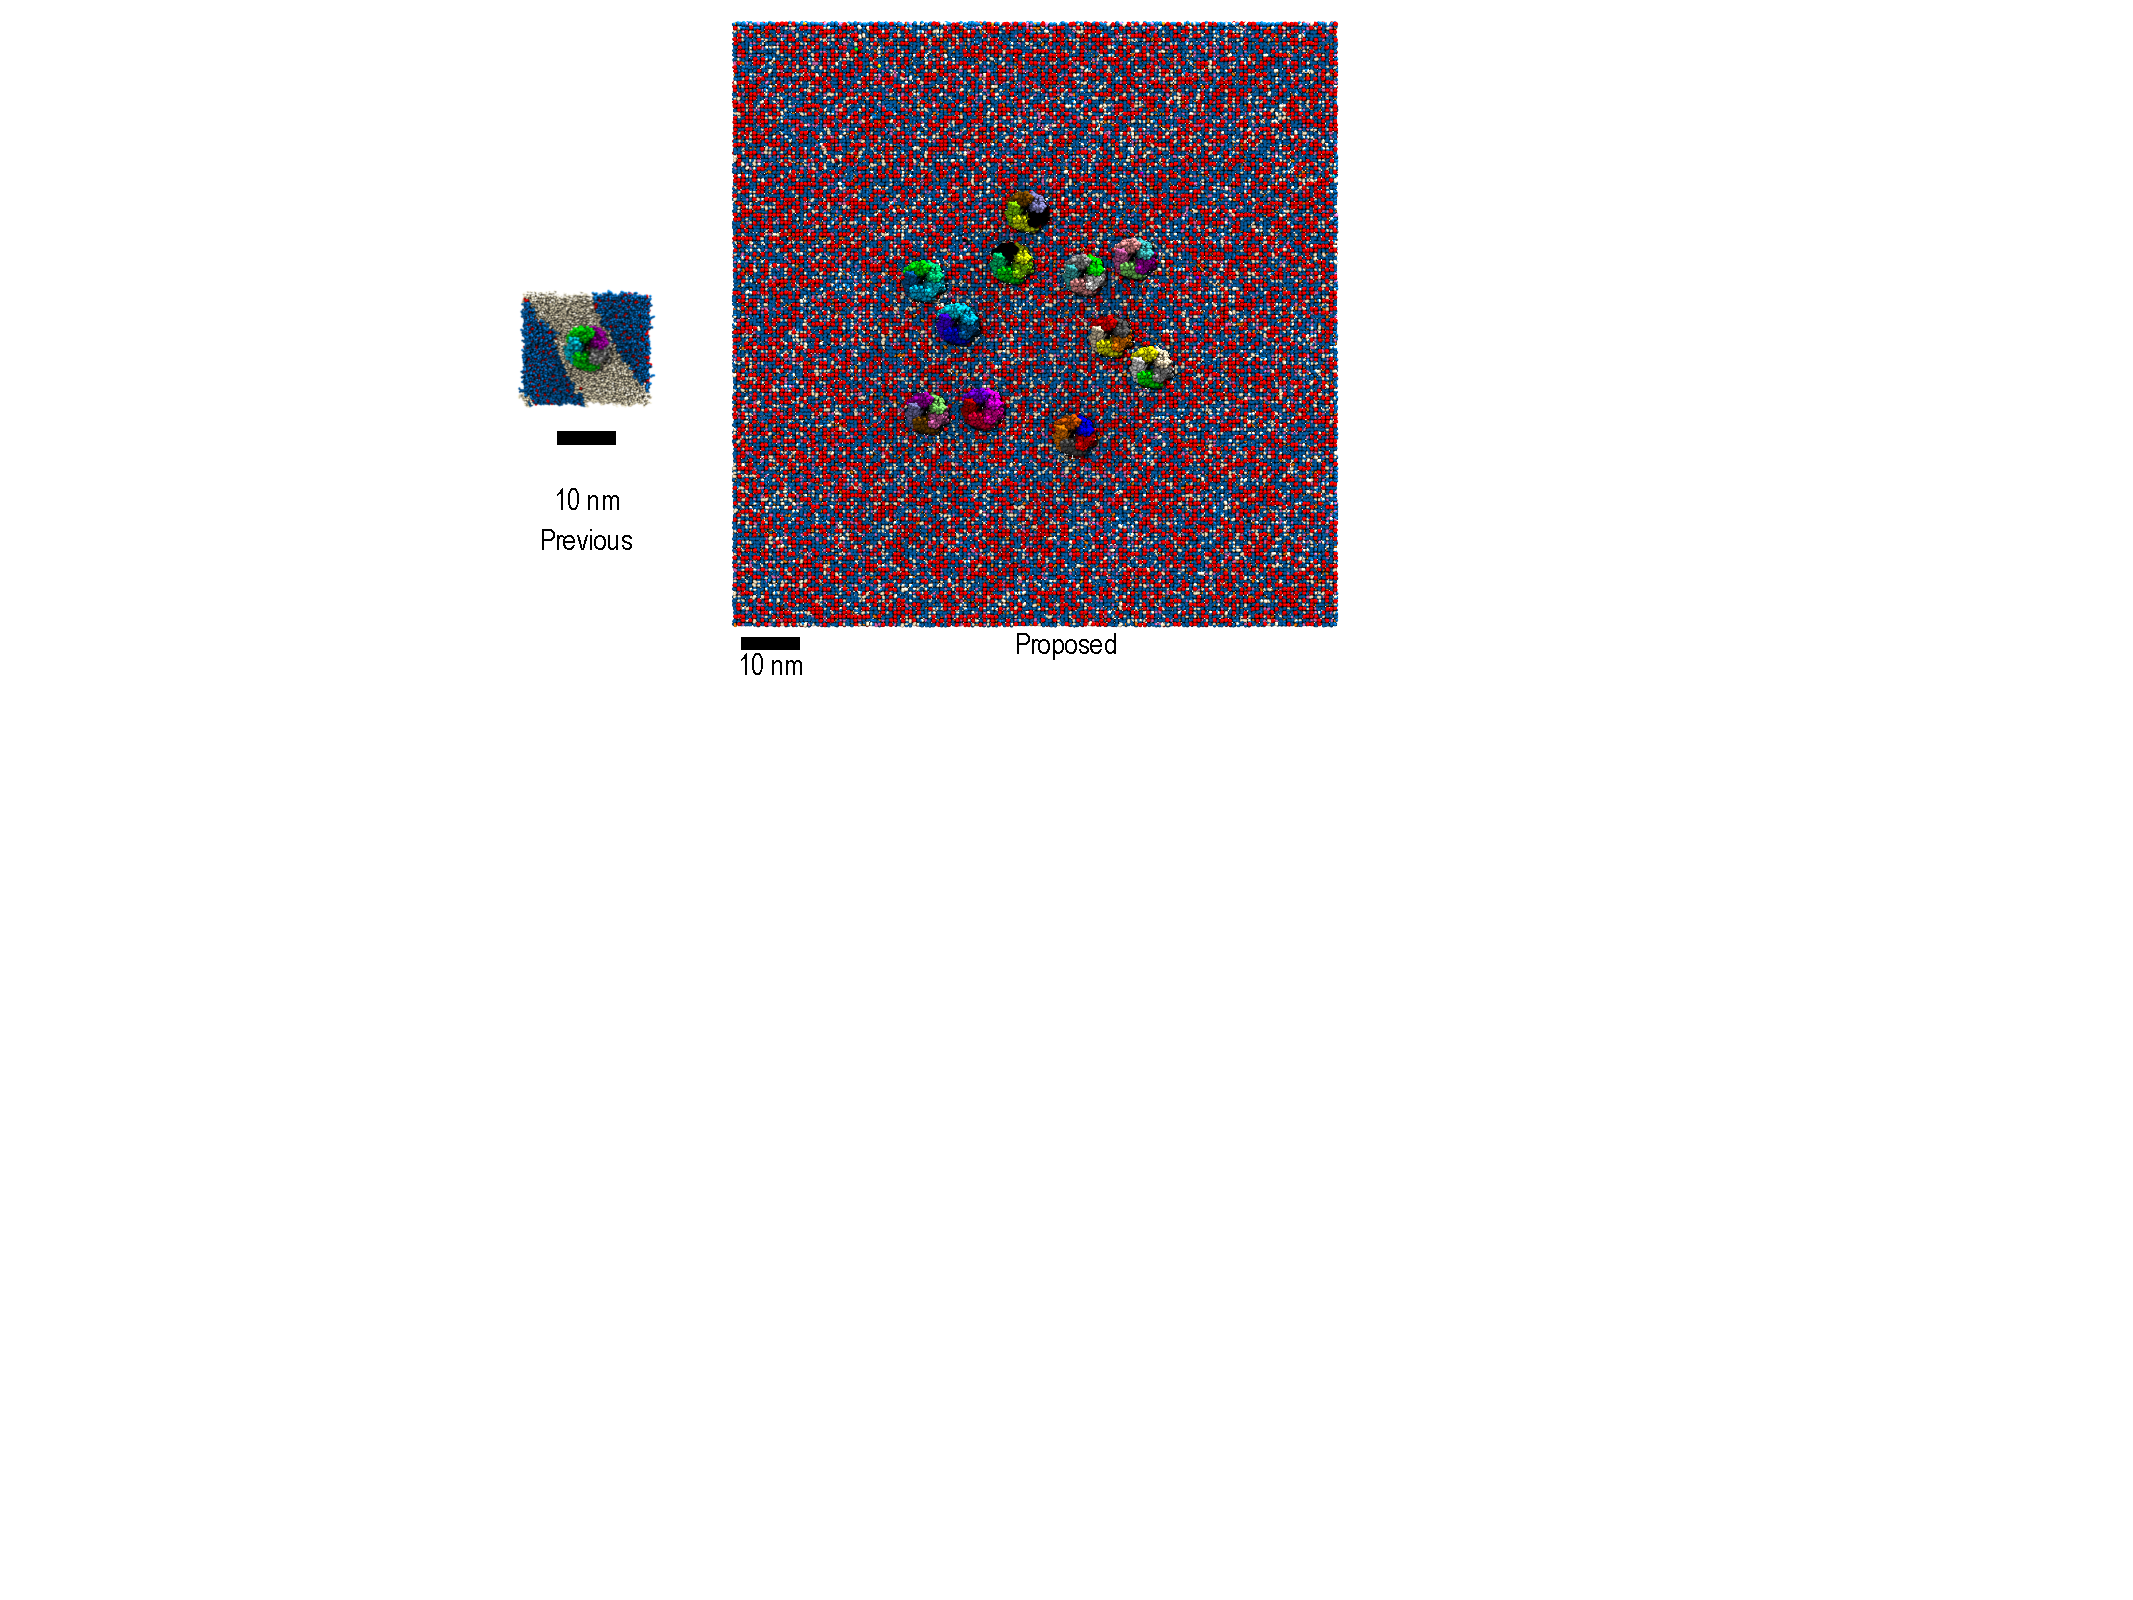
\includegraphics [scale=.4]{Science_Fig2.pdf}
\end{center}
\label{fig:Sci}
\caption{ Left: Previous simulation\cite{Sharp2019} run on Caliburn involving a domain-forming membrane with three different types of lipids and a neuronal ion channel. Right: A membrane of the size planned for simulation, comprising 1-10\% of the area of the post-synaptic membrane, and containing eleven of the same proteins.}
\end{figure}

%This research is motivated by two major questions:
%\begin{itemize}
%    \item Western diets are rich in omega-6 but low in omega-3 PUFAs. Does this lack of omega-3's change the organization of proteins in the post-synaptic membrane?
%    \item Membranes de-mix into two over-arching phases, one rich in cholesterol/saturated fatty acids and the other rich in unsaturated fatty acids. How do these domains change the distribution and density of proteins?
%\end{itemize}

%\subsection*{General Workflow}

{ \bf General Workflow} Our general pipeline is as follows:1) Construct system on local machine. Membranes will contain $\pmb{>30}$ \textbf{lipid species} in a composition similar to synapse by Ingolfson et al 2017\cite{Ingolfsson2017a}, and will also contain approximately \textbf{100 proteins} chosen from the most prevalent post-synaptic membrane proteins with available PDB structures. 2) Upload to Caliburn. 3) Run energy minimization and MD simulation using GROMACS 2019.2 \cite{Berendsen1995} for at least 20$\mu$s 4) Analyze using Visual Molecular Dynamics 1.9.3 \cite{HUMP96} and Python3. 
%Initial tests using membranes with $0.01\mu$m$^2$ in area, as in Figure 1B, have shown simulations run well with a time step of $0.02 ps$. The size of these simulations will require approximately  $\pmb{20 \mu s}$ to simulate each, the first $5-10 \mu s$ will be allowing the system to reach equilibrium. 
This research would require running 10 simulations with proteins and multiple lipid compositions, and 4 simulations without proteins , treated as controls. The net simulation time will be $\pmb{\sim 280 \mu s}$. \\

%\subsection*{Software Requirements and Storage.}

{\bf Software Requirements and Storage} The proposed research would utilize \textbf{GROMACS 2019.2 mpi packages } \cite{Berendsen1995} using the MARTINI 2.2\cite{Marrink2007} coarse grained force field.  Initial bench marking projects a single simulation will require 1 TBs of storage. For 14 simulations this would require \textbf{$\sim$ 3.0 TBs} of storage.\\

%\subsection*{Application Readiness}

{\bf Application Readiness} All software required is open-source and available on Caliburn.\\ %Systems lacking proteins can be prepared for simulation before the end of June. Membrane-proteins systems will require  about a month of testing in-order to optimize restraints. Caliburn currently has the software and packages for this research, available.

\section*{Number of requested SUs and storage justification}

{\bf Total number of SUs and storage, job size, scalability}
\begin{figure}[h]
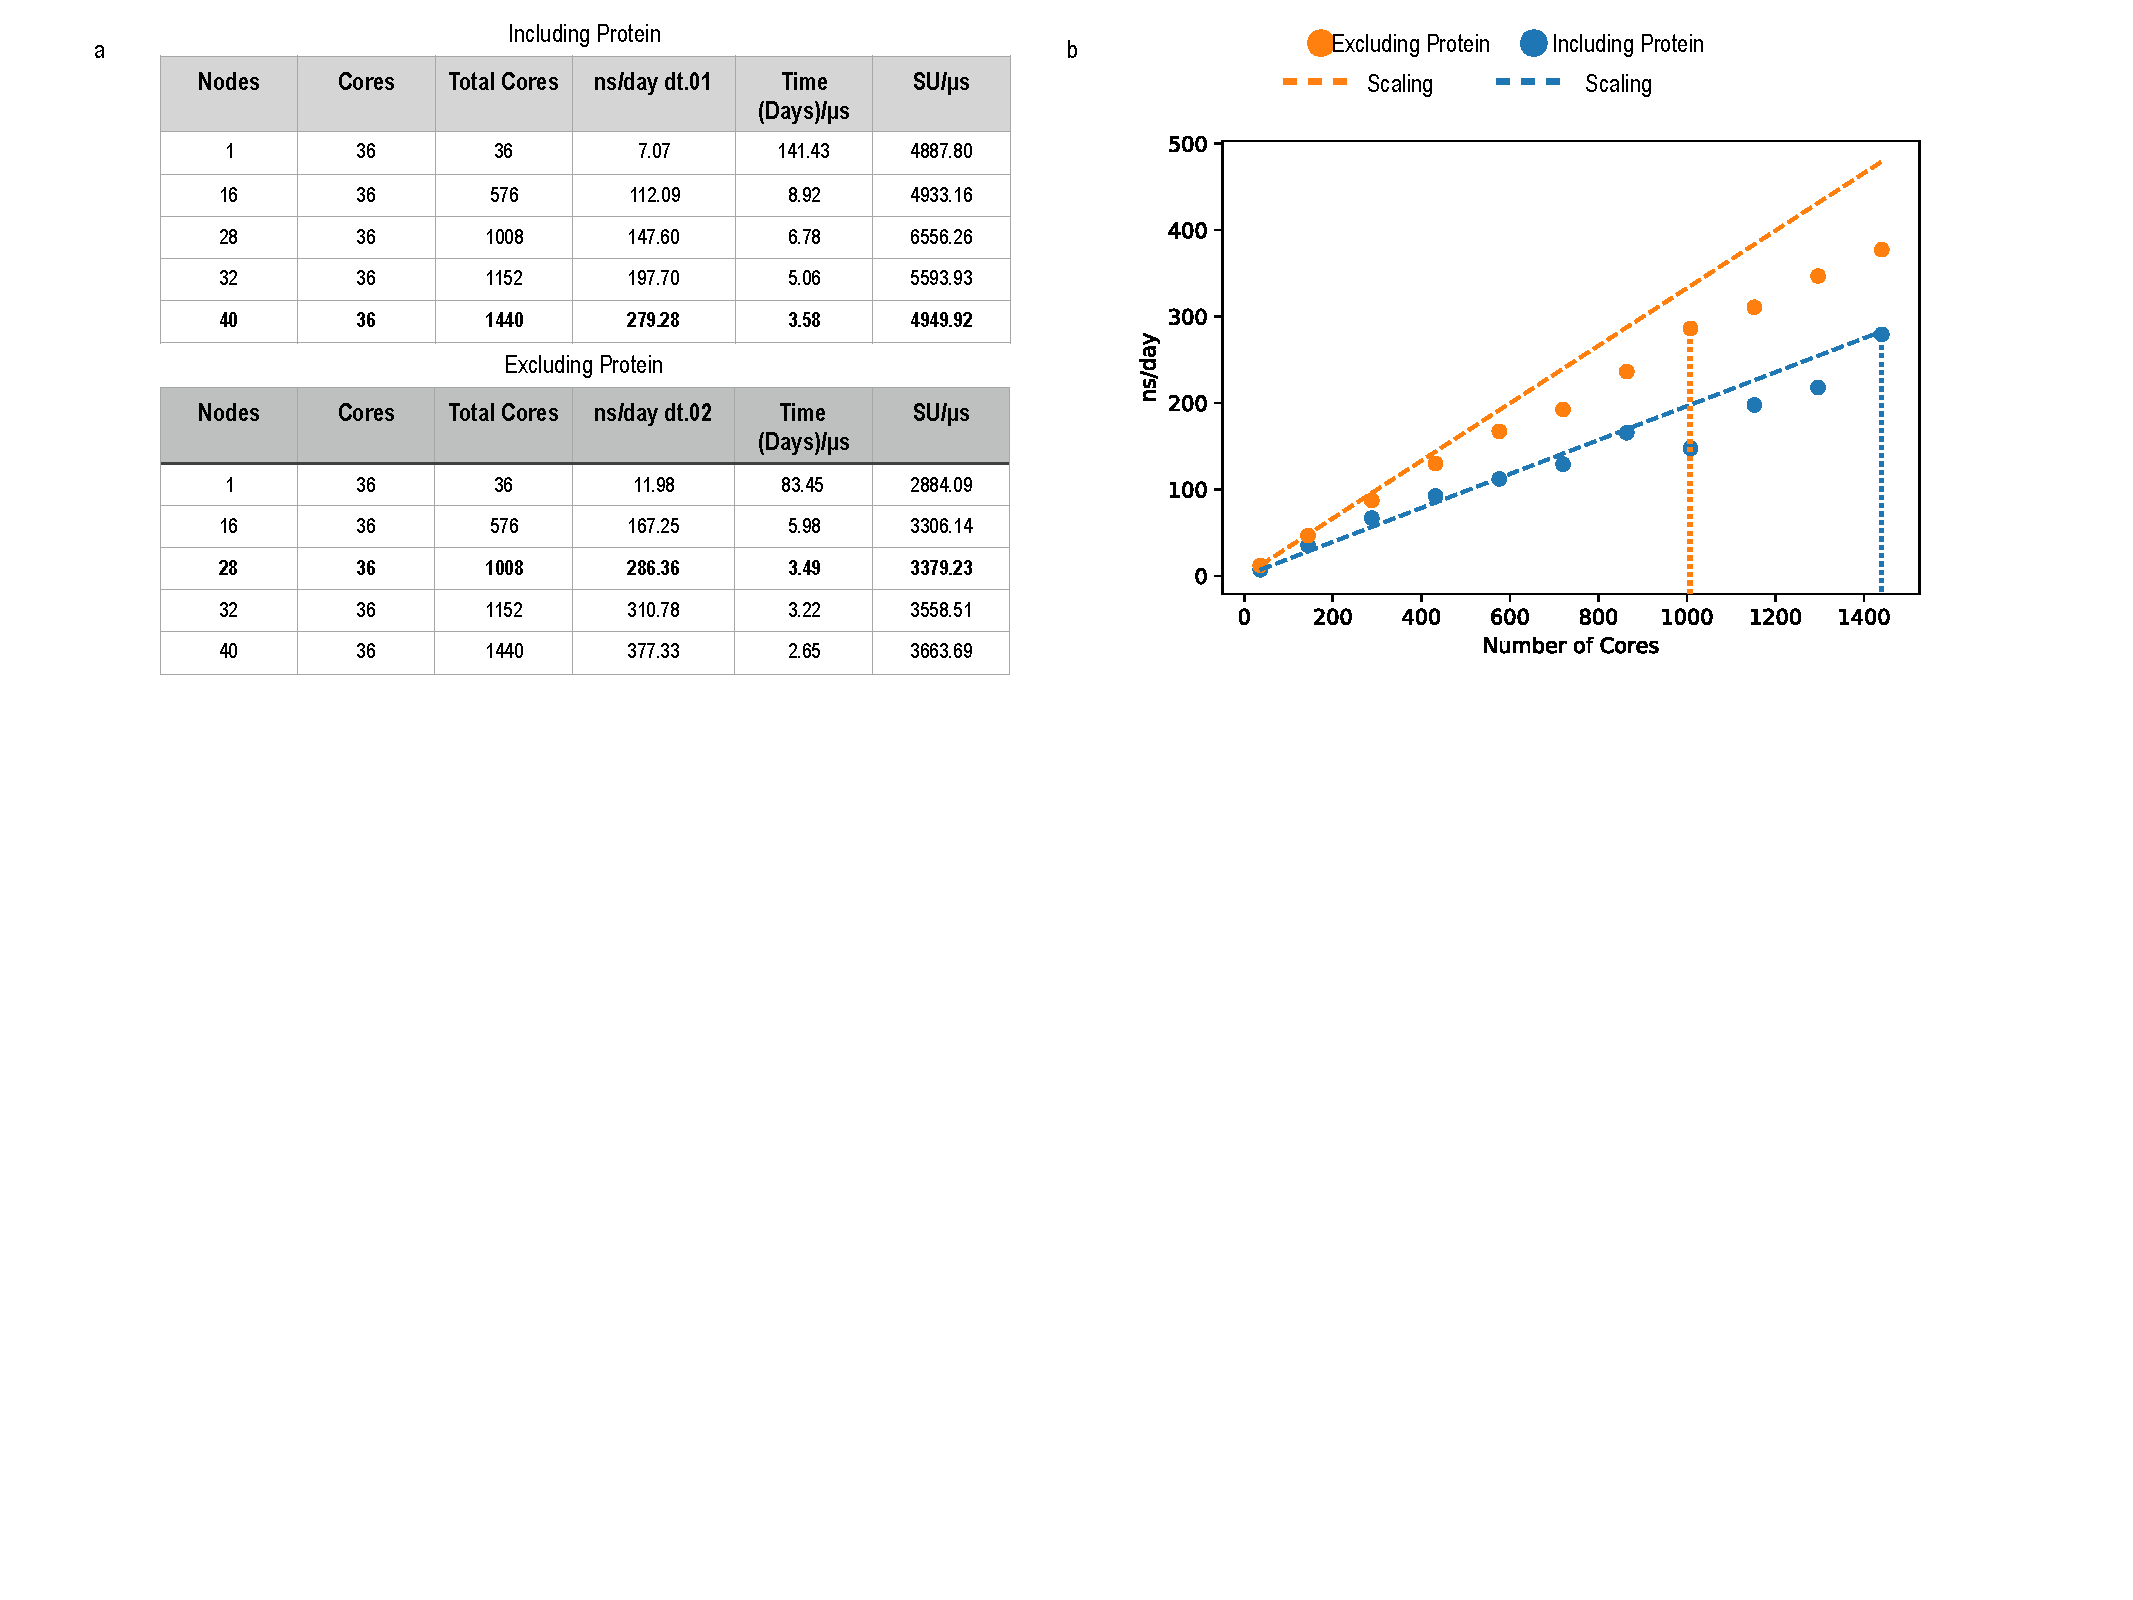
\includegraphics [scale=.5]{SU_Bench.pdf}
\label{fig:SU}
\caption{Projected SU's required for an iteration of membrane simulations with and without proteins. Bench marks are for systems with $\pmb{\> 8,000,000}$ \textbf beads a) Tables show subset of bench marked data. Systems including proteins showed 40 nodes and 36 cores provided the highest efficiency. Systems excluding proteins were tested using 28 cores and 36 nodes. These settings appear optimal to complete simulations within the allotted 6 months allocation. b) Full bench mark set comparing the ns/day to the total number of cores. Lines are associated with optimal node numbers.}
\end{figure}

Using Rutgers Offic of Advanced Research Computing Caliburn, \textbf{40 nodes and 36 cores} provided the best scaling for membranes with protein inclusions, and \textbf{28 nodes and 36 cores} for membrane only. We do observe $\sim 17\%$ divergence from expected scaling in membrane only systems, and a divergence for $\sim 1.25\%$ in the membrane-protein systems, while using 40 nodes and 36 cores Figure \ref{fig:SU}. \\

Membranes including proteins SU's:
\[20,000\textrm{ ns x }40\textrm{ nodes x }24\textrm{ hr/day x } 36 \textrm{ cores/node x } 1 \textrm{ SU/hr/node $ \div$ }279.3 \textrm{ ns/day = } \textbf{2,474,960 \textrm{SU}} \]
Membranes excluding proteins SU's:
\[ 20,000\textrm{ ns x }28\textrm{ nodes x }24\textrm{ hr/day x } 36 \textrm{ cores/node x } 1 \textrm{ SU/hr/node $ \div$ }377.3\textrm{ ns/day = } \textbf{2,413,732 \textrm{SU}} \]

For all systems we would need 34,404,528 SU's for this project: 

\[\textrm{Net SU's:  } (10*2,474,960 \textrm{ SU's}) + (4*2,413,732 \textrm{ SU's}) = \textbf{34,404,528 \textrm{ SU's}} \]

Systems are projected to require $\sim$ 4-5 months. to reach 20 $\mu s$. All simulations will produce upwards of $\sim$~1.0 TBs of data. For 14 systems this is a projected {14 TBs of data}, but most will be downloaded to local storage.  We request \textbf{3.0 TB} of working storage on Caliburn for this project.  \\

{\bf Access to Additional Resources}
We have access to Rutgers Office of Advanced Research Computing's Amarel, including maximum priority on 12 nodes. Due to the condominium structure of Amarel, it is not practical to continually run the massively parallel simulations we aim to run here, which requires 28 to 40 nodes.\\

\section*{Progress Report}

{\bf Publications From Previous Allocation}
\begin{itemize}
    \item \textit{The Structural Basis for Low Conductance in the Membrane Protein VDAC upon β-NADH Binding and Voltage Gating}, Cell Press, 2020 Raphael Böhm, Giuseppe Federico Amodeo, Sruthi Murlidaran, Shashank Chavali, Gerhard Wagner, Mathias Winterhalter, Grace Brannigan, Sebastian Hiller

    \item \textit{A lipid site shapes the agonist response of a pentameric ligand-gated ion channel}, Nature Chemical Biology, 2019, Camille M Hénault, Cedric Govaerts, Radovan Spurny, Marijke Brams, Argel Estrada-Mondragon, Joseph Lynch, Daniel Bertrand, Els Pardon, Genevieve L Evans, Kristen Woods, Benjamin W Elberson, Luis G Cuello, Grace Brannigan, Hugues Nury, Jan Steyaert, John E Baenziger, Chris Ulens

    \item \textit{Azi-medetomidine: Synthesis and Characterization of a Novel α2 Adrenergic Photoaffinity Ligand}, ACS Chemical Neuroscience, 2019, Andrew R McKinstry-Wu, Kellie A Woll, Thomas T Joseph, Weiming Bu, E Railey White, Natarajan V Bhanu, Benjamin A Garcia, Grace Brannigan, William P Dailey, Roderic G Eckenhoff

    \item \textit{Sequence specificity despite intrinsic disorder: How a disease-associated Val/Met polymorphism rearranges tertiary interactions in a long disordered protein}, PLoS Computaional Biology, 2019, Ruchi Lohia, Reza Salari, Grace Brannigan

    \item \textit{Untangling direct and domain-mediated interactions between nicotinic acetylcholine receptors in DHA-rich membranes}, The Journal of Membrane Biology, 2019, Kristen Woods, Liam Sharp, Grace Brannigan

    \item \textit{Competitive dewetting underlies site-specific binding of general anesthetics to GABA(A) receptors}, Pre-print, 2019, Sruthi Murlidaran, Jerome Henin, Grace Brannigan

    \item \textit{Direct Binding of Phosphatidylglycerol at Specific Sites Modulates Desensitization of a Pentameric Ligand-Gated Ion Channel}, eLife, 2019, Ailing Tong, John T Petroff, Fong-Fu Hsu, Philipp AM Schmidpeter, Crina M Nimigean, Liam Sharp, Grace Brannigan, Wayland WL Cheng

    \item \textit{Boundary lipids of the nicotinic acetylcholine receptor: spontaneous partitioning via coarse-grained molecular dynamics simulation}, Biochimica et Biophysica Acta (BBA)-Biomembranes, 2019, Liam Sharp, Reza Salari, Grace Brannigan
\end{itemize} \\

{\bf Projects In Continua}
\begin{itemize}
\item \textit{Boundary lipids of the nicotinic acetylcholine receptor in quasi-realistic native membrane}: We analyze our {\bf proposed neuronal membranes} to characterize boundary composition and specific protein-lipid occupancy sites. We embed nAChR within a quasi-native neuronal membrane and {\bf calculate the protein occupancy affinity} for our previously predicted lipid occupancy sites from model systems.

\item \textit{Using molecular dynamics simulations to elucidate a role for bacterial ceramides}: Sphingolipids synthesis was thought to be rare in Gram-negative bacteria, previously only found in a handful of taxa. We recently discovered ceramides in Caulobacter crescentus and demonstrated that these lipids play an important role in antibiotic and phage sensitivity. However, the mechanism by which {\bf ceramides affect resistance to antimicrobials}, as well as their effects on the {\bf integrity of the cell membrane are not yet clear. In this study, a {\bf coarse-grained molecular dynamics simulation} of a prototypical bacterial outer membrane} is used to observe changes in the conformation of the outer membrane lipids in the presence of ceramides. The outer membrane of a Gram-negative bacteria is asymmetric with an outer leaflet dominated by lipopolysaccharide (LPS). LPS is composed of three domains that extend from the outer membrane: a membrane-embedded lipid A, the attached core polysaccharide chain, and the O-antigen polysaccharide chain. A rough LPS consists of Lipid A and core chain only, while a smooth LPS contains Lipid A, core and O-antigen chains. Membranes were simulated with one to one ratio of rough to smooth LPS, with ceramide concentrations ranging from ten to forty percent of total lipids.  In order to understand the role of ceramide in outer membrane structure and function, this study considers their {\bf effects on the flexibility of O-antigen} as well as the {\bf clustering and packing of LPS} and membrane lipids.

\item \textit{Coronavirus envelope protein: lipid sensitivity and membrane bending}: {\bf The Coronavirus envelope (E) protein} is a pentameric viroporin that is implicated in numerous viral processes including but not limited to assembly, budding, envelope formation, and pathogenesis. While much work has recently been done to characterize this protein’s structure, function, and interactions with other proteins, its interactions with and effects on surrounding membranes are less well understood. It is known that the viroporin loses ion-selectivity in an exclusively neutral lipid environment, but it is not clear what drives this behavior. In the present study we {\bf use coarse-grained molecular dynamics (CG-MD) simulations to identify stable binding sites for anionic lipid head groups}. We then {\bf use all-atomistic molecular dynamics (AA-MD) simulations to investigate the effect of lipid charge on viroporin structure} using the sites identified from CG-MD. Incorporation of anionic lipid species into the existing protein structure may explain the change in selectivity observed in previous studies, and could prove useful for groups pursuing drug development projects. The E protein is also required for membrane curvature – giving the virus its characteristic shape in the process – although the precise mechanism is unknown. {\bf Using CG-MD, we observe that the E protein bends the membrane} in simulations with lipid species that have long acyl chains. We find this effect is limited when shorter lipid species are used, which suggests it results from asymmetric mismatch between the viroporin transmembrane domain (TMD) and the thickness of a typical host membrane. This result has implications for viral pathogenesis, as induction of {\bf membrane curvature is one of the important viral processes} that leads to budding and further viral spread
\end{itemize}\\

{\bf Recent Presentations}
\begin{itemize}
    \item \textit{Coronavirus envelope protein: lipid sensitivity and membrane bending}, 2020, APS Mid-Atlantic Section {\bf Presentation|}, Jesse Sandberg
    \item \textit{Coronavirus envelope protein: lipid sensitivity and membrane bending}, 2020, CCIB-Seminar {\bf Presentation}, Jesse Sandberg
    \item \textit{Using molecular dynamics simulations to elucidate a role for bacterial ceramides}, CCIB-Seminar {\bf Presentation}, Anushriya Subedy
    \item \textit{Coronavirus envelope protein: lipid sensitivity and membrane bending}, 2020, {\bf Poster}, Jesse Sandberg
    \item \textit{Using molecular dynamics simulations to elucidate a role for bacterial ceramides}, {\bf Poster}, Anushriya Subedy
\end{itemize}\\

{\bf Major Results}:
The nicotinic acetylcholine receptors (nAChRs) are pentameric ligand gated ion channels (pLGICs) responsible for conducting cations across the neuronal plasma membrane, and stimulating an action potential throughout the mammalian nervous systems. nAChRs are modulated by their local lipid composition (boundary lipids), and require a specific boundary composition for function. One modulating lipid is cholesterol.  Significant research has gone into understanding exactly what boundary lipids are crucial for nAChR function, but it is still unclear: do the boundary lipids have a neutral or anionic charge? What are the highest acyl-chain affinity: saturated or unsaturated? We hypothesize twenty occupancy sites, with complex boundary compositions, rich in cholesterol and PUFAs. We compared both previously studied model and quasi-neuronal membranes to try and characterize boundary composition and specific protein-lipid occupancy sites. First, using simulations of model domain and non-domain forming polyunsaturated (PUFA) rich ternary membranes, we analyze the whether nAChR resides in a liquid order or disorder domain, and potential specific lipid occupancy sites. Second, using the bacterial protein, Erwinia ligand-gated ion channel, a pLGIC of the same family, we analyze the preferential occupancy of neutral and anionic lipids. Finally, bringing all of the previous studies together, we embedded nAChR within a quasi-native neuronal membrane and calculated the protein occupancy affinity for our previously predicted lipid occupancy sites, see Figure \ref{fig:update}.

\begin{figure*}[h]
\begin{center}
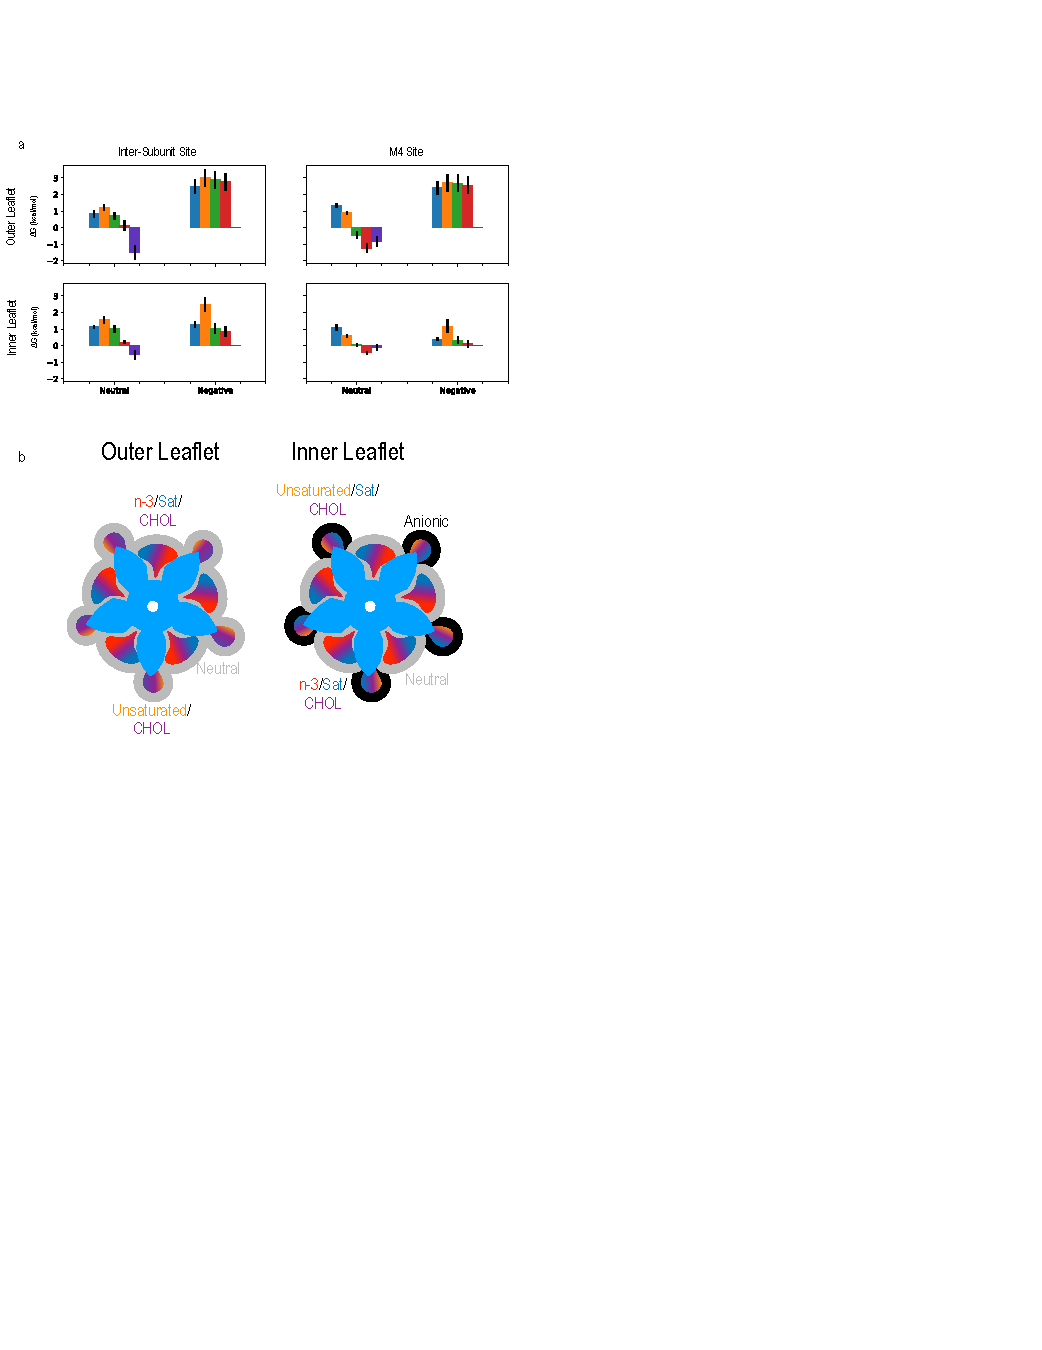
\includegraphics [width=\linewidth]{Caliburn_Udate.pdf}
\end{center}
\label{fig:update}
\caption{ Top: Free energy analysis comparing lipid binding sites by charge and lipid species. Bottom: Summary model of lipid distributions around a nicotinic acytlecholine receptor.}
\end{figure*}
\clearpage
\section*{Team Description}
    \begin{itemize}
    	\item PI: Dr. Grace Brannigan
	\begin{itemize}
	\item email address: gracebrannigan@gmail.com
	\item Contact Number: (856)-225-6780
	\item Address: JHSC 213, Rutgers Camden
	\item Campus: Rutgers Camden
	\item School: Rutgers Camden
	\item Department: Physics, CCIB
    \end{itemize}
    \end{itemize}
    Users:
        \begin{itemize}
        		\item Name: Liam Sharp
                \begin{itemize}       
			\item netid: lms464
                    	\item email address: lms464@scarletmail.rutgers.edu
                    	\item Contact Number: (609)-707-0974
                    	\item Address: JHSC 233, Rutgers Camden
                    	\item Campus: Rutgers Camden
                    	\item School: Rutgers Camden
                    	\item Department: CCIB
		\end{itemize}
		\item Name: Jesse Sandberg
	        \begin{itemize}
			\item netid: js2746
                    	\item email address: js2746@scarletmail.rutgers.edu
                    	\item Contact Number: (215)-470-7709
                    	\item Address: JHSC 233, Rutgers Camden
                    	\item Campus: Rutgers Camden
                    	\item School: Rutgers Camden
                    	\item Department: CCIB
	    \end{itemize}
	    \item Name: Tom Joseph
	    \begin{itemize}
	    		\item netid: tj227
                    	\item email address: ttjoseph@gmail.com
                    	\item Contact Number: (856)-571-4266
                    	\item Address: JHSC 233, Rutgers Camden
                    	\item Campus: Rutgers Camden
                    	\item School: Rutgers Camden
                    	\item Department: CCIB
	    \end{itemize}
	    \item Name: Anushriya Subedy
	    \begin{itemize}               
			\item netid: as3190
                    	\item email address: as3190@rutgers.edu
                    	\item Contact Number: (530)-848-2896
                    	\item Address: JHSC 233, Rutgers Camden
                    	\item Campus: Rutgers Camden
                    	\item School: Rutgers Camden
                    	\item Department: CCIB
	    \end{itemize}
	    \item Name: Connor Pitman
	    \begin{itemize}               
			\item netid: csp127
                    	\item email address: csp127@scarletmail.rutgers.edu
                    	\item Contact Number: (302)-893-5914
                    	\item Address: JHSC 233, Rutgers Camden
                    	\item Campus: Rutgers Camden
                    	\item School: Rutgers Camden
                    	\item Department: CCIB
	    \end{itemize}
	    \item Name: Jahmal Ennis
	    \begin{itemize}               
			\item netid: jje63
                    	\item email address: jje63@scarletmail.rutgers.edu
                    	\item Contact Number: (609)-353-7312
                    	\item Address: JHSC 233, Rutgers Camden
                    	\item Campus: Rutgers Camden
                    	\item School: Rutgers Camden
                    	\item Department: CCIB
	    \end{itemize}
	    \item Name: Mark Arcaria
	    \begin{itemize}               
			\item netid: ma1786
                    	\item email address: ma1786@scarletmail.rutgers.edu
                    	\item Contact Number: (215)-778-6251
                    	\item Address: JHSC 233, Rutgers Camden
                    	\item Campus: Rutgers Camden
                    	\item School: Rutgers Camden
                    	\item Department: CCIB
	    \end{itemize}

    \end{itemize}\printbibliography
\end{document}
